\chapter{Уравнения первого порядка, разрешённые относительно производной}

\section{Основные понятися и результаты}

\subsection{Объект изучения}

Рассмотрим обыкновенное дифференциальное уравнение первого порядка, разрешённое относительно проиводной:
\begin{equ}{1.1}
    \frac{\di y(x)}{\di x}, \qquad \text{или в краткой записи } y' = f(x, y)
\end{equ}

где $ x $ -- это независимая переменная, $ y = y(x) $ -- искомая функция, а $ f(x, y) $, \nimp, -- вещественная функция, определённая и непрерывная на множестве $ \vawe{G} = G \cup \hat{G} $, где:
\begin{itemize}
	\item $ G \sub \R^2 $ -- область
    \item $ \hat{G} \subseteq \partial G $ -- (возможно пустое) множество, на котором $ f(x, y) $ непрерывна или может быть доопределена с сохранением непрерывности
\end{itemize}

\begin{remind}
	Область -- связное открытое множество
\end{remind}

\begin{notation}
    $ G^* \define \partial G \setminus \hat{G} $
\end{notation}

\subsection{Решения дифференциального уравнения}

\begin{notation}
	Символ $ \langle $ подразумевает одну из скобок: $ ( $ или $ [ $, а символ $ \rangle $ -- скобку $ ) $ или $ ] $
\end{notation}

На вещественной оси рассмотрим непустое связное множество, не являющееся точкой. Это будет промежуток $ \braket{a, b} $

\begin{definition}
    Функция $ y = \vphi(x) $, заданная на промежутке $ \braket{a, b} $ называется решением дифференциального уравнения \eref{1.1}, если для любого $ x \in \braket{a, b} $ выполняются следующие три условия:
    \begin{enumerate}
        \item функция $ \vphi(x) $ дифференцируема
        \item точка $ \big( x, \vphi(x) \big) \in \vawe{G} $
        \item $ \vphi'(x) = f\big( x, \vphi(x) \big) $
    \end{enumerate}
\end{definition}

\begin{remark}
	График решения по определению не может состоять из одной точки
\end{remark}

\begin{remark}
	Первые два условия являются вспомогательными и позволяют записать третье
\end{remark}

\begin{remark}
    Любое решение является функцией не просто дифференцируемой а гладкой, т. е. $ \vphi(x) \in \Cont[1]{\braket{a, b}} $
\end{remark}

\begin{proof}
    Функция $ \vphi(x) $ дифференцируема (по условию 1). Значит, она непрерывна в любой точке $ x \in \braket{a, b} $ \\
    Значит, правая часть тождества из условия 3 непрерывна (как композиция непрерывных функций) \\
    Значит, и левая часть непрерывна \\
    При этом, если решение задано на отрезке $ [a, b] $, то на его концах существуют и непрерывны односторонние производные
\end{proof}

\begin{definition}
	Поскольку решение -- гладкая функция, то через люую точку $ \big( x, \vphi(x) \big) $ плоскости можно провести касательную под таким углом $ \alpha(x) $ с осью абсцисс, что $ \tg \alpha(x) = f \big(x, \vphi(x) \big) = \vphi'(x) $ \\
    Поэтому графики решений, имеющие общую точку соприкасаются в ней (``пересекаются под нулевым углом'')
\end{definition}

\begin{definition}
    Решение $ y = \vphi(x) $ уравнения \eref{1.1}, заданное на промежутке $ \braket{a, b} $ будем называть:
    \begin{itemize}
        \item внутренним, если $ \big( x, \vphi(x) \big) \in G $ для любого $ x \in \braket{a, b} $
        \item граничным, если $ \big( x, \vphi(x) \big) \in \hat{G} $ для любого $ x \in \braket{a, b} $
        \item смешанным, если найдутся такие $ x_1, x_2 \in \braket{a, b} $, что точка $ \big( x_1, \vphi(x_1) \big) \in G $, а точка $ \big( x_2 \vphi(x_2) \big) \in \hat{G} $
    \end{itemize}
\end{definition}

\begin{lemma}[о записи решения в интегральном виде]
    Для того чтобы определённая на промежутке $ \braket{a, b} $ функция $ y = \vphi(x) $ была решением дифференциального уравнения \eref{1.1}, необходимо и достаточно, чтобы функция $ \vphi(x) $ была непрерывна на $ \braket{a, b} $, её график лежал в $ \vawe{G} $ и при некотором $ x_0 \in \braket{a, b} $ выполнялос тождество
    \begin{equ}{1.2}
        \vphi(x) \overset{\braket{a, b}}\equiv \vphi(x_0) + \dint[s]{x_0}x{f\big( s, \vphi(s) \big)}
    \end{equ}
\end{lemma}

\begin{iproof}
	\item Необходимость \\
    Пусть функция $ y = \vphi(x) $ на $ \braket{a, b} $ является решением уравнения \eref{1.1} \\
    Тогда, по определению, справедливо тождество $ f\big( x, \vphi(x) \big) \overset{\braket{a, b}}\equiv \vphi'(x) $ \\
    Интегрируя его при любом фиксированном $ x_0 \in \braket{a, b} $ по $ s $ от $ x $ до $ x_0 $ и перенося $ \vphi(x_0) $ в правую часть, получаем тождество \eref{1.2}:
    $$ \dint[s]{x_0}x{f\big( s, \vphi(s) \big)} \overset{\braket{a, b}}\equiv \dint[s]{x_0}x{\vphi'(s)} = \vphi(x) - \vphi(x_0) $$
    \item Достаточность \\
    Пусть непрерывная на промежутке $ \braket{a, b} $ функция $ y = \vphi(x) $ удовлетворяет тождеству \eref{1.2} \\
    Тогда $ \vphi(x) $ непрерывно дифференцируема на $ \braket{a, b} $ (поскольку по \eref{1.2} она равна интегралу с переменным верхиним пределом от композиции непрерывных функций) \\
    Дифференцируя \eref{1.2}, заключаем, что выполняется и третье условие из определения решения
\end{iproof}

\subsection{Задача Коши}

\begin{problem}
    Для любой точки $ (x_0, y_0) \in \vawe{G} $ задача Коши с начальными данными $ x_0, y_0 $ заключается в том, чтобы найти все решения $ y = \vphi(x) $ уравнения \eref{1.1}, заданные на промежутках $ \braket{a, b} \ni x_0 $, в том числе внутренние, граничные или смешанные, такие что $ \vphi(x_0) = y_0 $ \\
    При этом говорят, что задача Коши поставлена в точке $ (x_0, y_0) $, а найденные решения -- это решения поставленной задачи Коши
\end{problem}

\begin{definition}
    Решение задачи Коши уравнения \eref{1.1} с начальными анными $ x_0, y_0 $ существует, если существует такое решение $ y = \vphi(x) $, определённое на промежутке $ \braket{a, b} \ni x_0 $, что $ \vphi(x_0) = y_0 $
\end{definition}

\begin{definition}
    Внутреннее (граничное, смешанное) решение задачи Коши с начальными данными $ x_0, y_0 $ существует, если точка $ (x_0, y_0) \in G(\hat{G}, \vawe{G}) $ и найдутся промежуток $ \braket{a, b} \ni x_0 $ и определённое на нём внутреннее (граничное, смешанное) решение $ y = \vphi(x) $ такие, что $ \vphi(x_0) = y_0 $
\end{definition}

\begin{definition}
    Задачу Коши, поставленную в точке $ (x_0, y_0) \in \vawe{G} $ будем называть
    \begin{itemize}
    	\item внутренней, если $ (x_0, y_0) \in G $
        \item граничной, если $ (x_0, y_0) \in \hat{G} $
    \end{itemize}
\end{definition}

\subsection{О существовании решения внутренней задачи Коши}

\begin{remind}
	Компакт в $ \R^n $ -- замкнутое ограниченное множество
\end{remind}

\begin{algorithm}[Пеано]
	Очевидно, что для любой точки $ (x_0, y_0) \in G $ найдутся такие константы $ a, b > 0 $, что прямоугольник
    $$ \ol{R} = \set{(x, y) : |x - x_0| \le a, ~ |y - y_0| \le b} $$
    являющийся компактом, лежит в области $ G $ \\
    Сразу исключим из рассмотрения простейший случай, когда $ f(x, y) \equiv 0 $ на $ \ol{R} $, в котором уравнение $ \eref{1.1} $ имеет решение $ y(x) \equiv y_0 $ при $ x \in [x_0 - a, x_0 + a] $ \\
    По второй теореме Вейерштрасса, $ f(x, y) $ достигает своего максимума на $ \ol{R} $. Положим
    $$ M \define \max\limits_{(x, y) \in \ol{R}}|f(x, y)| > 0, \qquad h = \min\set{a, \frac{b}M} \quad (h > 0) $$
\end{algorithm}

\begin{definition}
    Отрезок $ \ol{P_h}(x_0, y_0) = [x_0 - h, x_0 + h] $ называется отрезком Пеано, постоенным для точки $ (x_0, y_0) \in G $ \\
    Отрезки $ \ol{P_h^+}(x_0, y_0) = [x_0, x_0 + h] $ и $ \ol{P_h^-} = [x_0 - h, x_0] $ называются соответственно правым и левым отрезками Пеано
\end{definition}

\begin{theorem}[Пеано, о существовании внутреннего решения]\label{th:Peano}
    Пусть правая часть уравнения \eref{1.1} непрерывна в области $ G $. \\
    Тогда для любой точки $ (x_0, y_0) \in G $ и для любого отрезка Пеано $ \ol{P_h}(x_0, y_0) $ существует по крайней мере одно решение задачи Коши уравнения \eref{1.1} с начальными данными $ x_0, y_0 $, определённое на $ \ol{P_h}(x_0, y_0) $
\end{theorem}

\begin{proof}
	Будет доказано в \S2
\end{proof}

\subsection{Продолжимость решения}

\begin{definition}
    Пусть $ y = \vphi(x) $ -- решение уравнения \eref{1.1} на $ \braket{a, b} $. Если этот промежуток произвольным образом сузить, то на новом промежутке функция $ y = \vphi(x) $ останется решением, которое называют сужением исходного решения
\end{definition}

\begin{definition}
    Решение уравнения \eref{1.1}, заданное на промежутке $ \langle a, b) $ продолжимо вправо в точку $ b $ или на границу, если найдётся такое решение $ y = \vawe{\vphi}(x) $, определённое на промежутке $ \langle a, b] $, что сужение $ \vawe{\vphi}(x) $ на $ \langle a, b) $ совпадает с $ \vphi(x) $
\end{definition}

\begin{definition}
    Решение уравнения \eref{1.1}, заданное на промежутке $ \braket{a, b} $ продолжимо вправо за точку $ b $ или за границу, если найдутся такие $ \vawe{b} > b $ и решение $ y = \vawe{\vphi}(x) $, определённое на промежутке $ \braket{a, \vawe{b}} $, что сужение $ \vawe{\vphi}(x) $ на $ \braket{a, b} $ совпадает с $ \vphi(x) $
\end{definition}

\begin{theorem}[о продолжимости решения на границу]\label{th:cont}
    $ \vphi(x) $ -- решение уравнения \eref{1.1} на промежутке $ \langle a, b), \quad b < +\infty $ \\
    Для того чтобы это решение было продолжимо вправо в точку $ b $ необходимо и достаточно, чтобы существовали последовательность $ \seq{x_k}k $ и число $ \eta \in \R^1 $ такие, что
    \begin{equ}{1.3}
        \forall k \quad
        \begin{cases}
        	x_k \in \langle a, b) \\
            \bigg( x_k, \vphi(x_k) \bigg) \underarr{k \to \infty} (b, \eta) \in \vawe{G}
        \end{cases}
    \end{equ}
    Аналогично формулируется условие для продолжиомсти влево
\end{theorem}

\begin{iproof}
	\item Достаточность \\
    Пусть выполняется условие \eref{1.3}
    \begin{statement}
        В силу того, что функция $ f(x, y) $ определена и непрерывна на множестве $ \vawe{G} $, найдутся такие $ c > 0 $ и $ M \ge 1 $, что
        $$ \forall (x, y) \in \vawe{G} \cap \ol{B_c}(b, \eta) \quad |f(x, y)| \le M $$
    \end{statement}
    \begin{iproof}
        \item $ (b, \eta) \in G $, т. е. является внутренней \\
        Тогда существует $ \ol{B_c}(b, \eta) \sub G $ -- компакт, и на нём функция ограничена
        \item $ (b, \eta) \sub \vawe{G} $ и ``вблизи'' находятся точки ``плохой'' границы \\
        Приведём рассуждение \textbf{от противного}: \\
        Допустим, $ |f(b, \eta)| = M - 1 $ и существует последовательность $ c_m \underarr{m \to \infty} 0 $ ($ c_m > 0 $) и последовательность точек $ (x_m, y_m) \in \vawe{G} \cap \ol{B_{c_m}}(b, \eta) $ такие, что $ |f(x_m, y_m)| > M $ \\
        Тогда $ (x_m, y_m) \underarr{m \to \infty} (b, \eta) $, а это значит, что функция $ |f(x, y)| $ терпит разрыв в точке $ (b, \eta) $, так как $ |f(x_m, y_m)| - |f(b, \eta)| > 1 $ для любого $ m $
    \end{iproof}
    Докажем, что существует $ \liml{x \to b-} \vphi(x) $ и он равен $ \eta $: \\
    Для этого покажем, что для любого сколь угодно малого $ \veps > 0 $ найдётся число $ \delta \in \langle a, b) $, что
    \begin{equ}{1.4}
    	\forall x \in [\delta, b) : |\vphi(x) - \eta| < \veps
    \end{equ}
    Зафиксируем произвольный $ 0 < \veps \le c $ \\
    Тогда $ |f(x, y)| \le M $ для любой точки $ (x, y) \in \vawe{G} \cap \ol{B_\veps}(b, \eta) $ и по условию \eref{1.3} найдётся такой номер $ m $, что выполняются равентсва
    \begin{equ}{1.5}
        b - x_m > \frac\veps{2M}, \qquad |\vphi(x_m) - \eta| < \half[\veps]
    \end{equ}
    По формуле Ньютона-Лейбница для всякого $ x \in [x_m, b) $ имеем:
    \begin{multline*}
        |\vphi(x) - \vphi(x_m)| = \bigg| \dint[s]{x_m}x{\vphi'(s)}\bigg| = \bigg| \dint[s]{x_m}x{f \big( s, \vphi(s) \big)}\bigg| \le \dint[s]{x_m}x{|f \big( s, \vphi(s) \big)|} \le \\
        \le M(x - x_m) < M(b - x_m) \underset{\eref{1.5}_1}< \half[\veps] \qquad (x_m \le x < b)
    \end{multline*}
    Поэтому
    $$ |\vphi(x) - \eta| \le |\vphi(x) - \vphi(x_m)| + |\vphi(x_m) - \eta| \underset{\eref{1.5}_2}< \half[\veps] + \half[\veps] = \veps $$
    Неравенство \eref{1.4} верно при $ \delta = x_m $, а занчит, $ \vphi(x) \underarr{x \to b^{-0}} \eta $ \\
    Доопределим функцию $ y = \vphi(x) $ в точке $ b $, положив $ \vphi(b) = \eta $ \\
    Согласно \eref{1.2} $ \vphi(x) = \vphi(x_0) + \dint[s]{x_0}x{f \big(s, \vphi(s) \big)} $ для любых $ x_0, x \in \langle a, b) $ \\
    В этом тождестве можно перейти к пределу при $ x \to b^{-0} $, получая равенство $ \eta = \vphi(x_0) + \dint[s]{x_0}x{f \big( s, \vphi(s) \big)} $, так как по условию точка $ (b, \eta) \in \vawe{G} $, а занчит, функция $ f(x, y) $ определена и непрерывна в этой точке \\
    В результате функция
    $$ \vawe\vphi(x) =
    \begin{cases}
    	\vphi(x), \qquad x \in \langle a, b) \\
        \eta \qquad x = b
    \end{cases} $$
    по определению является продолжением решения $ y = \vphi(x) $ на $ \langle a, b] $
    \item Необходимость \\
    Допустим, что на промежутке $ \langle a, b] $ существует решение $ y = \vawe\vphi(x) $ такое, что $ \vawe\vphi(x) \equiv \vphi(x) $ на $ \langle a, b) $ \\
    Поскольку $ \vawe\vphi(x) $ непрерывна, то $ \vawe\vphi(x) = \eta = \liml{x \to b}\vawe\vphi(x) $ \\
    Но тогда $ \eta = \liml{x \to b^-}\vphi(x) $ и требуемая послеовательность точек $ x_k $ существует, причём по поределению решения точка $ (b, \eta) \in \vawe{G} $
\end{iproof}

\begin{lemma}[о продолжимости решения за границу отрезка]
    Пусть решение $ y = \vphi(x) $ уравнения \eref{1.1} определено на промежутке $ \langle a, b] $ и точка $ \big( b, \vphi(b) \big) \in G $ \\
    Тогда это решение продолжимо вправо за точку $ b $ на полуотрезок Пеано, построенный для точки $ \big( b, \vphi(b) \big) $
\end{lemma}

\begin{proof}
    По теореме Пеано (теор. \ref{th:Peano}) на отрезке Пеано $ \ol{P_h} \big( b, \vphi(b) \big) $ существует внутреннее решение $ y = \psi(x) $ задачи Коши с начальными данными $ \big( b, \vphi(b) \big) $ \\
    Тогда функция $ y = \vawe\vphi(x) $, где
    $$ \vawe\vphi(x) =
    \begin{cases}
        \vphi(x), \qquad x \in \langle a, b] \\
        \psi(x), \qquad x \in [b, b + h]
    \end{cases} $$
    по определению является решением уравнения \eref{1.1} на $ \langle a, b + h] $ \\
    В самом деле, в точке $ b $ производная функции $ \vawe\vphi(x) $ существует, так как
    $$ \vawe\vphi_-'(b) = \vphi_-'(b) = f \big( b, \vphi(b) \big) = \psi_+'(b) = \vawe\psi_+'(b) $$
    А выполнение других условий из определения решения для $ \vawe\vphi(x) $ очевидно
\end{proof}

Утверждение о продолжимости решения, определённого на промежутке $ [a, b \rangle $, влево за точку $ a $ формулируется аналогично

\begin{implication}
    Если решение $ y = \vphi(x) $ уравнения \eref{1.1} определено на промежутке $ \langle a, b] $ и не продолжимо вправо за точку $ b $, то $ \big( b, \vphi(b) \big) \in \hat{G} $ \\
    А если оно определено на промежутке $ [a, b \rangle $ и не продолжимо влево за точку $ a $, то $ \big( a, \vphi(a) \big) \in \hat{G} $
\end{implication}

\begin{proof}
	Предположение противного противоречит лемме
\end{proof}

Из теоремы о продолжимости решения на границу и последней леммы вытекает следующее утверждение:

\begin{lemma}[о продолжимости решения на границу интервала]
    Пусть решение $ y = \vphi(x) $ уравнения \eref{1.1} определено на промежутке $ \langle a, b) $, существует число $ \eta = \liml{x \to b^-}\vphi(x) $ и точка $ (b, \eta) \in G $ \\
    Тогда это решение продолжимо вправо за точку $ b $
\end{lemma}

Утверждение о продолжимости решения, заданного на $ (a, b \rangle $, влево за точку $ a $ формулируется аналогично

\subsection{Полное решение, интегральная кривая}

\begin{definition}
	Решение называется полным, или максимально продолженным, или непродолжимым в случае, если его нельзя продолжить ни влево, ни вправо, или что то же самое, когда оно не является сужением никакого другого решения
\end{definition}

\begin{definition}
	Внутреннее (граничное) решение называется полным, если его нельзя продолжить ни влево, ни вправо так, чтобы оно осталось внутренним (граничным)
\end{definition}

\begin{definition}
    Промежуток, на котором определено полное решение, бедм называть максимальным интервалом существования и обозначим $ I_{\max} $, а если для полного решения была поставлена задача Коши с начальными данными $ x_0, y_0 $, то $ I(x_0, y_0) $
\end{definition}

Из леммы о продолжимости решения за границу отрезка с очевидностью вытекает следующий факт:
\begin{statement}
	Максимальный интервал существования любого внутреннего решения -- это интервал
\end{statement}

\begin{theorem}[о существовании полного решения]\label{th:exist}
    Любое решение уравнения \eref{1.1} может быть продолжено до полного решения
\end{theorem}

\begin{restate}
    Любое решение уравнения \eref{1.1}, не являющееся полным, является сужением некоторого полного решения
\end{restate}

\begin{proof}
	Приведено в дополнении $ 1_4 $
\end{proof}

\begin{definition}
    График полного решения будем называть интегральной кривой уравнения \eref{1.1} \\
    Дуга интегральной кривой -- это график решения, заданного на любом промежутке $ \braket{a, b} \subsetneq I_{\max} $
\end{definition}

Таким образом, интегральные кривые уравнения \eref{1.1} лежат в $ \vawe{G} $, не могут иметь вертикальных касательных и не могут пересекаться под ненулевым углом, т. е. могут только соприкасаться

\begin{theorem}[о поведении интегральной кривой полного внутреннего решения]
    Предположим, что внутреннее решение $ y = \vphi(x) $ уравнения \eref{1.1} определено на промежутке $ \langle a, \beta) $ и не продолжимо вправо. \\
    Тогда для любого компакта $ \ol{H} \sub G $ найдётся такое число $ \delta \in \langle a, \beta) $, что для всякого $ x \in (\delta, \beta) $ точка $ \big( x, \vphi(x) \big) \in G \setminus \ol{H} $
\end{theorem}

\begin{restate}
	При стремлении аргумента полного внутреннего решения к границе максимального интервала существования дуга интегральной кривой покидает любой компакт, лежащий в области $ G $, и никогда в него не возвращается
\end{restate}

\begin{proof}
    Переходя в условиях теоремы на язык последовательностей, докажем, что для любого компакта $ \ol{H} \sub G $ и для любой последовательности $ x_k \underarr{k \to \infty} \beta $, $ x_k \in \langle a, \beta) $ существует $ K > 0 $ такое, что $ \big( x_k, \vphi(x_k) \big) \in G \setminus \ol{H} $ при всех $ k > K $ \\
    Рассуждая \textbf{от противного}, допустим, что существуют компакт $ \ol{H}_* \sub G $ и последовательность $ x_k \to \beta $, $ x_k \in \langle a, \beta) $ такие, что $ \big( x_k, \vphi(x_k) \big) \in \ol{H}_* $ для $ k = 1, 2, ... $ \\
    Отсюда сразу же вытекает, что $ \beta < +\infty $, так как в противном случае найдётся такой индекс $ k^* $, что точка $ \big( x_{k^*}, \vphi(x_{k^*}) \big) $ будет лежать вне компакта в силу его ограниченности \\
    НУО считаем, что последовательность $ x_k $ -- сходящаяся (иначе перейдём к сходящейся подпоследовательности) \\
    Пусть $ (\beta, \eta) = \limi{k} \big( x_k, \vphi(x_k) \big) $ \\
    Тогда предельная точка $ (\beta, \eta) $ также принадлежит компакту $ \ol{H}_* $, а значит, выполняются условия теоремы о продолжимости решения (теор. \ref{th:cont}), согласно которой решение $ y = \vphi(x) $ продолжимо на промежуток $ \langle a, \beta] $ -- \contra с условием теоремы
\end{proof}

Аналогичный результат имеет место для внутреннего решения, определённого на $ (\alpha, b \rangle $ и непродолжимого влево

\subsection{Вопросы, связанные с единственностью решения}

\begin{definition}\label{def:uniq:1}
    Точка $ (x_0, y_0) \in \vawe{G} $ называется точкой неединственности, если существуют такие решения $ y = \vphi_1(x) $ и $ y = \vphi_2(x) $ задачи Коши уравнения \eref{1.1} с начальными данными $ x_0, y_0 $, определённые на промежутке $ \braket{a, b} $, и такая последовательность $ x_k \infarr{k} x_0 $, $ x_k \in \braket{a, b} $, что $ \vphi_1(x_k) \ne \vphi_2(x_k) \quad (k = 1, 2, ...) $ \\
    В противном случае точка $ (x_0, y_0) $ называется точкой единственности
\end{definition}

\begin{remark}
    Любая точка граничного множества $ \hat{G} $, в которой решение задачи Коши отсутствует, по определению будет точкой единственности
\end{remark}

\begin{definition}\label{def:uniq:2}
    Точка $ (x_0, y_0) \in \vawe{G} $ называется точкой неединственности, если найдутся такие решения $ y = \vphi_1(x) $ и $ y = \vphi_2(x) $ задачи Коши уравнения \eref{1.1} с начальными данными $ x_0, y_0 $, определённые на $ \braket{a, b} $, что
    $$ \forall (\alpha, \beta) \ni x_0 \quad \exist x^* \in (\alpha, \beta) \cap \braket{a, b} : \quad \vphi_1(x^*) \ne \vphi_2(x^*) $$
\end{definition}

\begin{statement}
	Определения точки неединственности равносильны
\end{statement}

\begin{iproof}
    \item опр. \ref{def:uniq:1} $ \implies $ опр. \ref{def:uniq:2} \\
    Из опр. \ref{def:uniq:1} вытекает, что для всякого интервала $ (\alpha, \beta) \ni x_0 $ найдётся такой индекс $ k^* $, что $ x_{k^*} \in (\alpha, \beta) $, поэтому в опр. \ref{def:uniq:2} $ x^* = x_{k^*} $
    \item опр. \ref{def:uniq:2} $ \implies $ опр. \ref{def:uniq:1} \\
    Можно выбрать последовательность интервалов $ (\alpha_k, \beta_k) $, которая с ростом $ k $ стягивается в точку $ x_0 $. Тогда по опр. \ref{def:uniq:2} для всякого $ k $ найдётся $ x_k^* \in (\alpha_k, \beta_k) \cap \braket{a, b} $, что $ \vphi_1(x_k^*) \ne \vphi_2(x_k^*) $, т. е. $ x_k^* $ -- последовательность из опр. \ref{def:uniq:1}
\end{iproof}

Отрицая опр. \ref{def:uniq:2}, получаем ``прямое'' определение точки единственности:
\begin{definition}
    Точку $ (x_0, y_0) \in \vawe{G} $ будем называть точкой единственности в следующих случаях:
    \begin{enumerate}
        \item задача Коши уравнения \eref{1.1} с начальными данными $ x_0, y_0 $ не имеет решений
        \item для любых двух решений $ y = \vphi_1(x) $ и $ y = \vphi_2(x) $ этой задачи Коши, определённых на некотором промежутке $ \braket{a, b} $, найдётся интервал $ (\alpha, \beta) \ni x_0 $ такой, что
        $$ \forall x \in (\alpha, \beta) \cap \braket{a, b} \quad \vphi_1(x) = \vphi_2(x) $$
    \end{enumerate}
\end{definition}

\begin{note}
	Здесь надо иметь в виду следующее:
    \begin{itemize}
    	\item Если $ (x_0, y_0) \in G $:
        \begin{itemize}
        	\item Случай 1 не может возникнуть
            \item По теореме Пеано (теор. \ref{th:Peano}) все решения задачи Коши определены на отрезке Пеано $ [x_0 - h, x_0 + h] $ ($ h > 0 $) \\
            Поэтому в определении точки единственности для любых двух решений достаточно требовать наличия интервала $ (\alpha, \beta) \ni x_0 $, на котором они совпадают
        \end{itemize}
        \item Если $ (x_0, y_0) \in \hat{G} $ и, например, решение нельзя продолжить за точку $ x_0 $ вправо, то в определнии для любых двух решений задач Коши при их наличии надо потребовать существования промежутка $ (\alpha, x_0] $, на котором они совпадают
    \end{itemize}
\end{note}

\begin{definition}
    Решение задачи Коши уравнения \eref{1.1}, поставленной в точке $ (x_0, y_0) \in \vawe{G} $ называется:
    \begin{itemize}
    	\item неединственным, если $ (x_0, y_0) $ -- точка неединственности
        \item единственным в точке, если оно сущетвует и $ (x_0, y_0) $ -- точка единственности
    \end{itemize}
\end{definition}

\begin{definition}
    Решение внутренней задачи Коши уравнения \eref{1.1}, поставленной в точке $ (x_0, y_0) $ называется локально единственным, если существует интервал $ (\alpha, \beta) \ni x_0 $ такой, что все решения этой задачи продолжимы на $ (\alpha, \beta) $ и для любых двух её решений $ y = \vphi_1(x) $ и $ y = \vphi_2(x) $, при необходимости произвольным образом продолженных на $ (\alpha, \beta) $, имеем $ \vphi_1(x) \equiv \vphi_2(x) $ на $ (\alpha, \beta) $
\end{definition}

\begin{theorem}pо локальной единственности решения внутренней задачи Коши]
	Пусть $ (x_0, y_0) \in G $ -- это точка единственности \\
    Тогда решение задачи Коши уравнения \eref{1.1} с начальными данными $ x_0, y_0 $ является локально единственным
\end{theorem}

\begin{proof}
	Будет доказано в \S4, п. $ 1^0 $
\end{proof}

\begin{implication}
	Из этой теоремы вытекает, что для внутренней задачи Коши понятия единственности решения в точке и локальной единственности равносильны
\end{implication}

\subsection{Достаточные условия единственности}

\begin{definition}
    Будем говорить, что решение задачи Коши $ y = \vphi(x) $, поставленное в точке $ (x_0, y_0) \in \vawe{G} $ и определённое на промежутке $ \braket{a, b} \ni x_0 $, единственно на этом промежутке, или, просто, единственно, если для любого $ x \in \braket{a, b} $ точка $ \big( x, \vphi(x) \big) $ является точкой локальной единственности
\end{definition}

\begin{definition}
    Область $ G^0 \sub G $ будем называть областью единственности для уравнения \eref{1.1}, если каждая точка $ G^0 $ является точкой единственности. Множество $ \vawe{G^0} = G^0 \cup \hat{G^0} $, в котором $ \hat{G^0} $ -- это множество граничных точек $ G^0 $, являющихся точками единственности, будем называть множеством единсвтенности
\end{definition}

\begin{theorem}[о единственности; слабая]\label{th:uniq:weak}
    Пусть в уравнении \eref{1.1} функция $ f(x, y) $ определена и непрерывна в области $ G $, а частная производная $ \pder{f(x, y)}y $ определена и непрерывна в области $ G^0 \sub G $ \\
    Тогда $ G^0 $ является областью единственности
\end{theorem}

\begin{proof}
    Эта теорема является следствием более сильных теорем о единственности, которые будут свормулированы и доказаны в \S4, п. $ 4^0 $, причём не только для области $ G $, а для всего множества $ \vawe{G} $
\end{proof}

\subsection{Частные и особые решения}

\begin{definition}
    Решение уравнения \eref{1.1}, заданное на промежутке $ \braket{a, b} $, будем назвыать частным (особым), если его график состоит только из точек единственности (неединственности) и это решение является полным в том смысле, что не может быть продолжено ни влево, ни вправо так, чтобы его график состоял только из точек единственности (неединственности). В этом случае промежуток $ \braket{a, b} $ будем называть максимальным интервалом существования частного (особого) решения
\end{definition}

\subsection{Понятие общего решения}

\begin{definition}
    Общим решением уравнения \eref{1.1} на некотором связном множестве $ A^* $, лежащем в области единственности $ G^0 $, называется функция $ y = \vphi(x, C) $, определённая и непрерывная по совокупности аргументов на множестве $ Q_{A^*} = \set{(x, C) | x \in \braket{a(C), b(C)}, \quad C \in \braket{C_1, C_2}} $, если выполняются следующие два условия:
    \begin{enumerate}
    	\item для любой точки $ (x_0, y_0) \in A^* $ уравнение $ y_0 = \vphi(x_0, C) $ имеет единственное решение $ C = C_0 $
        \item функция $ y = \vphi(x, C_0) $ -- это решение задачи Коши уравнения \eref{1.1} с начальными данными $ x_0, y_0 $, определённое на промежутке $ \braket{a(C_0), b(C_0)} $
    \end{enumerate}
\end{definition}

\begin{theorem}[о существовании общего решения]\label{th:comm:exist}
    Для произвольной точки $ (x_0^*, y_0^*) $ из области единственности $ G^0 $ уравнения \eref{1.1} найдётся связное множество $ A^* : (x_0^*, y_0^*) \in A^* \sub G^0 $, на котором существует общее решение
\end{theorem}

\begin{proof}
	Приведено в \S5
\end{proof}

\subsection{Поле направлений и метод изоклин}

\begin{definition}
    Отрезок проивольной длины с центром в точке $ (x_0, y_0) \in \vawe{G} $ и тангенсом угла наклона, равным $ f(x_0, y_0) $, будем называть отрезком поля направлений, построенным в точке $ (x_0, y_0) $ \\
    Само множество $ \vawe{G} $, запоненное отрезками поля направлений будем называть полем направлений, индуцированным уравнением \eref{1.1}
\end{definition}

Кривая, лежащая в $ \vawe{G} $, является интегральной тогда и только тогда, когда она гладкая и в каждой точке направление касательной к ней совпадает с направлением поля в этой точке

\begin{definition}
    Изоклиной уравнения \eref{1.1} называется любая кривая, расположенная во множестве $ \vawe{G} $, в каждой точке которой направление поля имеет один и тот же угол наклона
\end{definition}

\begin{remark}
	Все изоклины задаются уравнением $ f(x, y) = k $, где $ k $ -- любое вещественное число из области значений $ f(x, y) $
\end{remark}

Метод изоклин заключается в том, чтобы, нарисовав достаточное число изоклин и отрезков поля на них, начертить характерные интегральные кривые, которые, опадая на очередную изоклину, должны касаться отрезков поля направлений, построенных на ней

\section{Существование решения внутренней задачи Коши}

В этом параграфе будет доказана теорема Пеано о существовании решения внутренней задачи Коши уравнения \eref{1.1} $ y' = f(x, y) $ (теор. \ref{th:Peano}), т. е. будет рассматриваться задача Коши, поставленная в любой внутренней точке $ \vawe{G} $, и строиться решение этой задачи, график которого лежит в области $ G $ \\
Будем строить решение при помощи ``метода ломаных Эйлера''

\subsection{Ломаные Эйлера}

\begin{wrapfigure}{l}{0.5\textwidth}
	\centering
    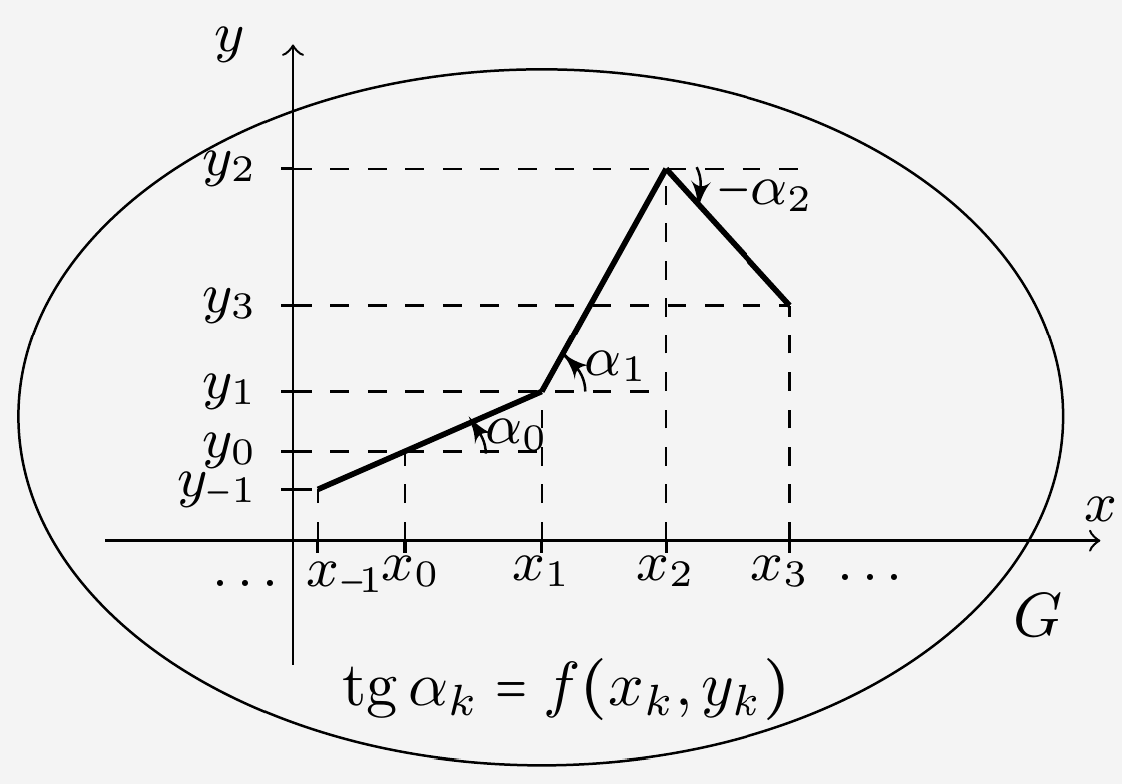
\includegraphics[scale=0.27]{euler-polylines}
\end{wrapfigure}

Выберем в области $ G $ произвольную точку $ (x_0, y_0) $ и построим в ней отрезок поля направлений столь малой длины, что он целиком лежит в $ G $, начинаясь в какой-то точке $ (x_{-1}, y_{-1}) $ и заканчиваясь в точке $ (x_1, y_1) $ \\
Проведём вправо через точку $ (x_1, y_1) $ и влево через точку $ (x_{-1}, y_{-1}) $ полуотрезки поля, лежащие в $ G $ и заканчивающиеся в точках $ (x_2, y_2) $ и $ (x_{-2}, y_{-2}) $ соответственно, и так далее \\
Этот процесс можно продолжать любое конечное число шагов $ N $, поскольку область $ G $ -- открытое множество \\
График полученной таким образом непрерывной кусочно-линейной функции $ y = \psi(x) $ называется ломаной Эйлера \\
Итак, установлено, что ломаная Эйлера лежит в области $ G $, проходит через точку $ (x_0, y_0) $ и абсциссы её угловых точек равны $ x_j $ ($ j = \ol{-N, N} $)

\begin{definition}
	Рангом дробления ломаной Эйлера назовём число, равное
    $$ \max\limits_{j = \ol{1 - N, N}}\set{x_j - x_{j - 1}} $$
\end{definition}

Формула, реккурентно задающая ломаную Эйлера $ y = \psi(x) $, иммеет вид: $ \psi(x_0) = y_0 $ и далее при $ j = 0, 1, ..., N - 1 $ для любого $ x \in (x_j, x_{j + 1}] $ или при $ j = 0, -1, ..., 1 - N $ для любого $ x \in [x_{j - 1}, x_j) $
\begin{equ}{1.8}
	\psi(x) = \psi(x_j) + f \big( x_j, \psi(x_j) \big)(x - x_j)
\end{equ}
В частности, при $ j = 0 $ отрезок ломаной Эйлера определён для любого $ x \in [x_{-1}, x_1] $ и, делясь на два полуотрезка, проходит через точку $ (x_0, y_0) $ под углом, тангенс которого равен $ f(x_0, y_0) $ \\
Из формулы \eref{1.8} вытекает, что для всякого $ j = \ol{0, N - 1} $ производная $ \psi'(x) = f \big( x_j, \psi(x_j) \big) $ при $ x \in (x_j, x_{j + 1}) $, а в точке $ x_{j + 1} $ она не определна, как и в точках $ x_{j - 1} $ при $ j \le 0 $ \\
Доопределим $ \psi'(x) $ в точках разрыва как левостороннюю производную при $ x > x_0 $ и как правостороннюю производную при $ x < x_0 $, положив
$$ \psi'(x_j) = \psi_{\mp}'(x_j) \liml{x \to x_j^{\mp0}}\frac{\psi(x) - \psi(x_j)}{x - x_j} \qquad (j = \pm 1. ..., \pm N) $$
А при $ j = 0 $ существует полная производная $ \psi'(x_0) = f(x_0, y_0) $ \\
Таким образом, для любого $ x \in (x_j, x_{j + 1}] $ ($ j = 0, 1, ..., N - 1 $) или для любого $ x \in [x_{j - 1}, x_j) $ ($ j = 0, -1, ..., 1 - N $), дифференцируя равенство \eref{1.8} по $ x $, получаем
\begin{equ}{1.9}
    \psi'(x) = f \big( x_j, \psi(x_j) \big), \qquad j \in \set{1 - N, ..., N - 1}
\end{equ}

\subsection{Лемма об \texorpdfstring{$ \veps $}e-решении}

Покажем, что на некотором промежутке всегда можно построить функцию, график которой проходит через заданную точку области $ G $, такую, что при подстановке этой функции в уравнение \eref{1.1} окажется, что разность между левой и правой частями уравнения по модулю не превосходит любого сколь угодно малого наперёд заданного положительного числа

\begin{definition}
    Для всякого $ \veps > 0 $ непрерывная и кусочно-гладкая на отрезке $ [a, b] $ функция $ y = \psi(x) $ называется $ \veps $-решением уравнения \eref{1.1} на $ [a, b] $, если для любого $ x \in [a, b] $ точка $ \big( x, \psi(x) \big) \in G $ и
    \begin{equ}{1.10}
    	\big| \psi'(x) - f \big( x, \psi(x) \big) \big| \le \veps
    \end{equ}
\end{definition}

\begin{lemma}[о ломаных Эйлера в роли $ \veps $-решения]
    Для любой точки $ (x_0, y_0) \in G $ и для любого отрезка Пеано $ \ol{P_h}(x_0, y_0) $ имеем:
    \begin{enumerate}
        \item Для любого $ \delta > 0 $ на $ \ol{P_h} $ можно построить ломаную Эйлера $ y = \psi(x) $ с рангом дробления, не превосходящим $ \delta $, график которой лежит в прямоугольнике $ \ol{R} $ \nimp[из определения отрезка Пеано]
        \item Для любого $ \veps > 0 $ найдётся такое $ \delta > 0 $, что всякая ломаная Эйлера $ y = \psi(x) $ с рангом дробления, не превосходящим $ \delta $, является $ \veps $-решением уравнения \eref{1.1} на $ \ol{P_h}(x_0, y_0) $
    \end{enumerate}
\end{lemma}

\begin{proof}
	\hfill
    \begin{enumerate}
        \item Для произвольной точки $ (x_0, y_0) $ из $ G $ построим прямоугольник $ \ol{R} \sub G $ с центром в $ (x_0, y_0) $ и два лежащих в нём равнобедренных треугольника $ \ol{T^-}, \ol{T^+} $ с общей вершиной в точке $ (y_0, x_0) $ и основаниями, параллельными оси ординат, как это было сделано при построении отрезка Пеано \\
        При этом зафиксируются константы $ a, b, M, h $ \\
        Выберем $ \delta_* < \delta $ так, чтобы число $ \frac{h}{\delta_*} \fed N \in \N $ \\
        Положим $ x_{j + 1} \define x_j + \delta_* $ ($ j = \ol{0, N - 1}) $, тогда $ x_N = x_0 + h $ \\
        Для всякого $ x > x_0 $ будем последовательно строить отрезки ломаной Эйлера $ y = \psi(x) $ с узлами в точках $ x_j $ \\
        Для любого $ j = 0, ..., N $ это сделать возможно, так как модуль тангенса укла наклона каждого отрезка равен $ \big| f \big(x_j, \psi(x_j) \big) \big| $, а тангенсы углов наклона боковых сторон треугольника $ \ol{T^+} $ по построению равны $ \pm M $, где $ M = \max|f(x, y)| $ на компакте $ \ol{R} $ \\
        Поэтому любой отрезок ломаной Эйлера, начиная с первого, не может пересечь боковую стенку $ \ol{T^+} $, а значит, содержится в нём \\
        В результате для всех $ x \in [x_0, x_0 + h] $ точка $ \big( x, \psi(x) \big) \in \ol{T^+} $ и требуемая ломаная Эйлера построена на $ [x_0, x_0 + h] $ \\
        Для левого отрезка Пеано всё аналогично
        \item Зафиксируем теперь произвольное положительное число $ \veps $ \\
        Функция $ f(x, y) $ непрерывна на компакте $ \ol{R} $, следовательно, по теореме Кантора $ f $ равномерно непрерывна на нём. По определнию это занчит, что существует такое $ \delta_1 > 0 $, что для любых двух точек $ (x' y') $ и $ (x'', y'') $ из прямоугольника $ \ol{R} $ таких, что $ |x' - x''| \le \delta_1 $ и $ |y' - y''| < \delta_1 $, выполняется неравенство $ |f(x', y') - f(x'', y'')| \le \veps $ \\
        Положим $ \delta \define \min\set{\delta_1, \frac{\delta_1}M} $ и покажем, что для любой ломаной Эйлера $ y = \psi(x) $ с рангом дробления меньшим, чем $ \delta $ на отрезке Пеано $ \ol{P_h}(x_0, y_0) = [x_0 - h, x_0 + h] $, справедливо неравенство \eref{1.10}: \\
        Возьмём любую точку $ x $ из отрезка Пеано, например справа от $ x_0 $ \\
        Найдётся индекс $ j \in \set{0, ..., N - 1} $ такой, что $ x \in (x_j, x_{j + 1}] $, т. е. $ x_j $ -- ближайшая к $ x $ левая угловая точка ломаной Эйлера \\
        Согласно \eref{1.9}
        $$ \psi'(x) - f \big(x, \psi(x) \big) = f \big( x_j, \psi(x_j) \big) - f \big( x, \psi(x) \big) $$
        Оценим близость аргументов функции $ f $: \\
        По выбору $ \delta $ и $ j $ имеем
        $$ |x - x_j| \le \delta \le \delta_1, \qquad |\psi(x) - \psi(x_j)| \undereq{\eref{1.8}} \big| f \big( x_j, \psi(x_j) \big) \big| \cdot |x - x_j| \le M\delta \bdef[\le]\delta \delta_1 $$
        Поэтому из равномерной непрерывности функции $ f $ вытекает, что
        $$ \big| f(x_j, \psi(x_j) \big) - f \big( x, \psi(x) \big) \big| \le \veps $$
        А значит, неравенство \eref{1.10} из определения $ \veps $-решения выполняется на отрезке Пеано
    \end{enumerate}
\end{proof}

\subsection{Лемма Арцела-Асколи}

Пусть последовательность функций $ \seq{h_n(x)}n $ задана на $ [a, b] $

\begin{definition}
    Каждая из функций последовательности $ \seq{h_n(x)}n $ ограничена на $ [a, b] $, если
    $$ \forall n \ge 1 \quad \exist K_n > 0 : \quad \forall x \in [a, b] \quad |h_n(x)| \le K_n $$
\end{definition}

\begin{definition}\label{def:clamp:eq}
    Последовательность $ \seq{h_n(x)}n $ \bt{равномерно} ограничена на отрезке $ [a, b] $, если
    $$ \bm{\exist K > 0} : \quad \forall n \ge 1 \quad \forall x \in [a, b] \quad |h_n(x)| \le K $$
\end{definition}

\begin{definition}
    Каждая из функций последовательности $ \seq{h_n(x)}n $ непрерывна на отрезке $ [a, b] $, значит, согласно теореме Кантора, равномерно непрерывна на $ [a, b] $, если
    $$ \forall \veps > 0 \quad \forall n \ge 1 \quad \exist \delta_n > 0 : \quad \forall x', x'' \in [a, b] \quad \nimp[\bigg(] |x' - x''| \le \delta_n \implies |h_n(x') - h_n(x'')| \le \veps \nimp[\bigg)] $$
\end{definition}

\begin{definition}\label{def:cont:eq}
    Последовательность $ \seq{h_n(x)}n $ \bt{равностепенно} непрерывна на отрезке $ [a, b] $, если
    $$ \forall \veps > 0 \quad \bm{\exist \delta > 0} : \quad \forall n \ge 1 \quad \forall x', x'' \in [a, b] \quad \nimp[\bigg(] |x' - x''| \le \delta \implies |h_n(x') - h_n(x'')| \le \veps \nimp[\bigg)] $$
\end{definition}

\begin{definition}
    Последовательность функций $ \seq{h_n(x)}n $ поточечно сходится к некоторой функции $ h(x) $ на отрезке $ [a, b] $, если
    $$ \forall \veps > 0 \quad \forall x \in [a, b] \quad \exist N_x > 0 : \quad \forall i, j \ge N_x \quad |h_i(x) - h_j(x)| \le \veps $$
\end{definition}

\begin{definition}\label{def:lim:eq}
    Последовательность $ \seq{h_n(x)}n $ \bt{равномерно} сходится к некоторой функции $ h(x) $ на отрезке $ [a, b] $, если
    $$ \forall \veps > 0 \quad \bm{\exist N > 0} : \quad \forall i, j \ge N \quad \forall x \in [a, b] \quad |h_i(x) - h_j(x)| \le \veps $$
\end{definition}

\begin{notation}
	Для любого $ x \in [a, b] $ поточечная сходимость обозначается $ h_n(x) \to h(x) $
\end{notation}

\begin{notation}
    Равномерная относительно $ [a, b] $ сходимость обозначается $ h_n(x) \xrightrightarrows[x \to \infty]{[a, b]} h(x) $
\end{notation}

\begin{remark}
    В определениях \ref{def:clamp:eq} и \ref{def:cont:eq} слова ``равномерно'' и ``равностепенно'' означают, что константы $ K, \delta $ не зависят от выбора $ n $, а в \ref{def:lim:eq} -- что номер $ N $ не зависит от выбора $ x $
\end{remark}
